


\documentclass[12pt,a4paper]{article}

\usepackage[utf8]{inputenc}
\usepackage[american]{babel}
\usepackage[T1]{fontenc}
\usepackage{listings}
\usepackage{graphicx}

\title{NoWork\\ Personal Report}
\author{Inigo Mediavilla\\[2em]}
\date\today

\begin{document}
\maketitle

%% Index
%% - Introduction to Rewriting system (what it is, what is useful for)
%% - Justification for the project (what have we gained from doing,
%% how could a user benefit from it)
%%
%% - Global vision of the project (short description of how to
%% describe a language with the system, describing every one of the concepts)
%%
%% - Subsystems (a short description of every part
%% of the project (parsing, typechecking
%% - How does the system work? Explain how the rewriting of a system
%% is implemented by giving a term and explaining what is the term,
%% what is the pattern, what is the metavariable of placeholder
%% -
%% - Problem with rewriting (what subtree should I replace first -
%% show with an example why it matters because it affects the result)
%% - Initial Naive version of rewriting: (1. without fixpoint (Problems)
%% 2. Bottom-up and Top-down 3. Higher flexibility Strategies)
%%
%% - Conclusion

\section{Introduction to rewriting systems}

Term rewriting systems are systems that  are defined as a set of transformations called
rewriting rules. These rewriting rules are the core of the language and
they define the computational power of the language as well as
its expressivity and other properties.

 These systems have applications that are not
restricted to the well known general paradigm programming languages
for computers. Systems based on this kind of rules have been used for
the analysis of bussiness interactions or for the formalization of
some logics, for example the Brouwer-Heyting-Kolmogorov interpretation has shown that
predicate logic can be expressed as a set of rewriting rules.

One of the reasons why this kind of systems are so widely used is that
they have been well studied, they are well understood and a
wide range of tools exist to prove properties on them.

\section{Justification}

Despite the multiple applications of these systems and all the
mathematical tools available to prove properties on them building a
new rewriting system or tuning an existing one for experimentation is
still a really tedious task. The implementation of this kind of
system from scratch requires building a parser for the language, a
type checker, and all the code to find matches for a rule and
transforming the existing term when matches are found. Most of these
steps require a great amount of work even though they're relatively
simple. Besides a great amount of this work could be generalized since
the difference between two of these systems are reduced only to the
definition of the rules.

This is the purpose of Nowork, to provide the generic part in the
implementation of this kind of system allowing users to define new
systems by only defining the rules that define them.

%% It also allows to prove some properties on them and further work
%% on nowork could also facilitate the automatic verification of
%% properties for these systems.


\section{ NoWork - Rewriting System }

NoWork users can define their own rewriting system without having to
write their own parser, typechecker and whithout having to code the
reduction rules of the interpreter of the programming language. To do
that NoWork offers a language where all the rules can be defined as
well as all the types, constants and operations available in the
language.

Rules are defined as a pattern  and a transformation. The pattern
describes the model that NoWork will try to find in a given term
to replace it by the transformation specified by the rule.

\begin{figure}[!h]
\begin{center}
\begin{verbatim}

rule = pattern + transformation

rule [beta] :
  App(Lambda(?x, ?T), ?U)  => Subst(?x, ?T, ?U)

pattern = App(Lambda(?x, ?T), ?U) 
transformation = Subst(?x, ?T, ?U)

\end{verbatim}
\end{center}
\caption{Structure of a pattern}
\end{figure}

On top of that NoWork allows a simple syntax for defining Constants.

\begin{figure}[!h]
\begin{verbatim}

constant Nil : forall(A).List<A>
\end{verbatim}
\caption{Definition of a constant}
\end{figure}


It also allows to define Operators that are not like the higher order functions
that we know in functional programming languages since all the
reduction in NoWork is specified in the reduction rules. Operators
just give the name and the type of a reduction. Usually in the
definition of a language every operator will have a rewriting rule
that will take a subtree whose root has the same name as the operator
and if the language is well formed the transformation will conform to
the typing defined in the operator.


\begin{figure}[!h]
\begin{verbatim}

operator Cons : forall(A).A * List<A> -> List<A>

\end{verbatim}
\caption{Definition of an operator}
\end{figure}

Kinds allow to define the constant types and also the polymorphic types when
their definition depends on a type variable.

\begin{figure}[!h]
\begin{verbatim}

kind Bool : type // Constant type
kind List : type -> type // Polymorphic type
\end{verbatim}
\caption{Definition of kinds}
\end{figure}

Therefore, the rewriting rules provide the semantics of the language
while the type annotations provided in the constants, the operators as well
as the kinds allow the user to define the typing rules. All together
this language helps the user concisely define a programming language
declaratively without having to implement a parser, a typechecker and
an interpreter.

\section{Global vision of the system}

We can consider that code written in NoWork belongs to one of two
different categories:

Definitions of the language. Written in NoWork's language. Contains the
constants, operators, kinds and rules as they have been described
previously. This definition must conform to the grammar and type
checking rules of NoWork's language to avoid the definition of
malformed languages.

Language Terms. Once a language has been defined with NoWork terms of
that language can be written as trees. This trees should conform to the
typing rules that have been defined for the language that are
independent of NoWork's language rules.

In addition NoWork provides a mini-language with a list of commands that are parsed by
NoWork's toplevel and that allow the user to interact with the
program. When the toplevel receives command it executes a list of
steps that can be generalized to:

\subsection{Process}

The process by which NoWork can define new rewriting systems and
evaluate terms in a rewriting system can be reduced to the following steps:

\begin{figure}[!h]
\begin{verbatim}
Parsing + Type Checking  + Rewriting
Rewrting = pattern matching + transformation
\end{verbatim}
\caption{ Phases of the evaluation of a command }
\end{figure}

Parsing: This step reads a string and converts it to an AST that
can contain a definition of a language or an interaction with a term
of the language

Typechecking: If the command is a definition of the language NoWork's
Language typing rules are verified. Otherwise the command is an interaction with a
term and the term needs to be typed checked against the definition of
the language contained in the environment.

Rewriting: This phase occurs only when the command is not a definition
of the language. In this phase the term is explored with a
given strategy looking for matches of the patterns described in the
rewriting rules of the language. When a match is found the
transformation is applied to the part of the term where the match
was found.

\section{Rewriting}

Rules are defined as patterns with placeholders (look for the name for
that) . When a match is found the placeholders act as variables whose
values are given by the content of the match. Those variables can be
reused in the transformation. In a simple version of pattern matching
called linear pattern matchin they act like capture groups in regular
expresions. (Beware that NoWork has implemented a more complex version of
pattern matching called non-linear pattern matching where the same
placeholder can appear many times in the same pattern).

For example if we take again the initial example we can see the
pattern, placeholder and transformation in a rule of lambda calculus.

\begin{figure}
\begin{verbatim}
App(Lambda(?x, ?T), ?U) => Subst(...)

Pattern = App(Lambda(?x, ?T), ?U)
Transformation = Subst(?x, ?T, ?U)
Placeholders = {x, T, U}

When applied to:

App(Lambda(a, a), b)
Environment = { x = a, T = a, U = b }

\end{verbatim}
\caption{Elements of a pattern}
\end{figure}

During the rewriting process the rewriting mechanism asks the pattern
matcher to look for matches of a pattern and the pattern matcher
returns the matches with the values for the placeholders. Once the
rewriting process has it only has to fill the holes that exist in the
transformation with the values of the environment generated from the
matching.


\begin{figure}
\begin{verbatim}
Environment = { x = a, y = a, z = b }

Subst (x, y, z ) in Environment => Subst (a, a, b) 

\end{verbatim}
\caption{Rewriting last step}
\end{figure}

However this really simple vision of rewriting hides a small subtlety
that concerns the way the term is traversed during pattern matching
and how the transformations are applied. The initial problem is that
a term can have many occurrences of the same match and depending on
how the tree is traversed the result of applying the same set of rules
may be different.


\begin{figure}[!h]
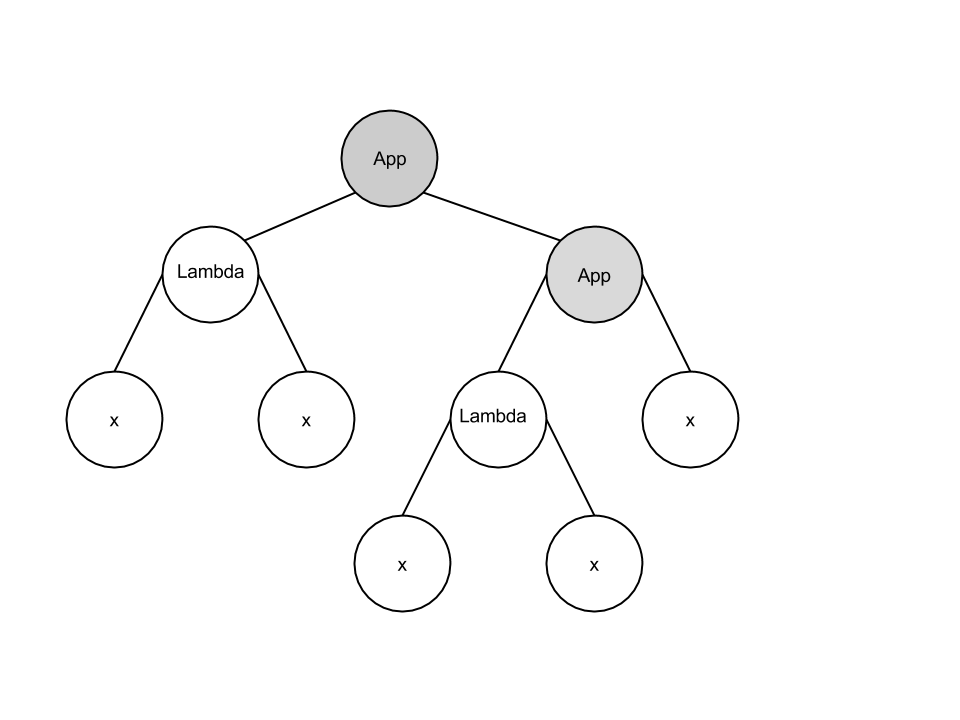
\includegraphics[scale=0.4]{multiple-reductions.png}

\caption{Term with different reductions}
\label{multiple-reductions}
\end{figure}

In figure~\ref{multiple-reductions} we can see how there are two possible reductions that are marked with
a darker background. Either the reduction can happen at the root of
the tree or the reduction can happen in the application that happens
on the right child of the root. In this case if we keep
reducing until we get to an irreducible term the result will be the
same independently of which one of those reductions we apply
first. However there are cases where the reduction order can have an
effect in the final result, for example there exist terms in lambda
calculus that converge when the strategy chosen is call by value
whereas they would reduced to an irreducible term when call by name is
used. 

On top of that as a user that is experimenting with a new language we
may want to trace the reduction of terms using different evaluation
orders.

Thus, NoWork needed to provide different reduction strategies and to
allow the user to choose which one will be used when a reduction happens.

\subsection{Strategies}

The simplest solution to this problem consists on predefining the
strategy to explore the tree looking for matches and coding the
rewriting algorithm to respect this strategy. This was the approach
that was implemented in the first versions of NoWork and the initial
strategies that were implemented where Bottom-up where matches are
found starting from the bottom of the tree and climbing the tree and
Top-down that does the opposite.

However the project required the implementation of more
strategies and the solution that was adopted was the definition of a
language of strategies that allows the user to specify the way the
rewriting algorithm traverses the term to rewrite it. A good
explanation of the language of strategies is provided in NoWork's user
manual. 
\section{Conclusion}

We have seen that programming languages have many applications not
only in computer science but also in other fields like logic and the
analysis of business processes for example. However the implementation
of programming languages for the verification of some of their
properties is a long process even if some of the steps could be
simplified and generalized. That is the purpose of NoWork, to simplify
the process of creating a naive version of a programming language just
by describing the rewriting rules and the typing rules of the
language. Once this is done the user can test the reduction of a term
given its AST.


We have also seen a quick description of what is the process that is
carried out inside NoWork to allow the user to define a language and
try to reduce a term of the language to then explain more in depth the
implementation process for the rewriting part of the process. We have
seen the importance of the evaluation order in the matches and how in
NoWork started by implementing two simple hardcoded strategies
Top-Down and Bottom-Up to then provide a more powerful and flexible
solution based on a minilanguage for the description of strategies.

The resulting implementation of NoWork is a tool that allows to
define languages in a simple way and that provides a flexible language
to specify the evaluation strategy for the language. Therefore it
could prove a really valuable tool for defining prototype languages
and manually verify some reduction properties on them.

From a pedagogical point of view the implementation of nominal
workbench has provided me with a deeper understanding of rewriting,
considering this concept in Peano Arithmetic, or CCS has widened the
vision that I had for this concept mainly reduced to lambda calculus
at the beginning of the project.


%\subsection{ Pedagogical value }
%What have I learned, What are the disadvantages and advantages of the
%solution proposed, how could this implementation could be improved in
%the future...

%Problem:

%Defining a framework for writing nominal rewriting systems:

%Why? Because it is useful to play with different variations of a
%rewriting systems to understand the differences in expressivity, ``puissance'',
%congruence, and normalisation properties

%(Describe every one of those properties)

%This kind of tool with the right support for traces and the right level of explanation in every
%operation can be a powerful learning tool.

%Why nominal and non-linera? The additional adjectives of non-linear and nominal 


%The initial implementation

%- Is Kleene's algorithm necessary to reduce terms to their normal form
%- Problems with rewriting systems
%  - alpha conversion + difficulty to do proofs

\end{document}
